\chapter {Materials and Methods}

The objective of this study was to measure and quantify MRI-induce translational and torque forces experienced by an  post-surgical epicardial pacing leads when exposed to the static magnetic field. Safety limits for MRI magnetic fields are well established and described in the Introduction, based on ASTM F-series guidelines. Following these methods, we constructed non-magnetic test apparatus specifically designed to measure these forces with the precision required for clinical applications.

However, clinical access for experimental testing posed a significant challenge, as MRI scanner time is typically associated with long scheduling delays and short available measurement periods. Therefore, a secondary objective of this work was to improve the quality of our experimental setup in order to maximize the efficiency of data acquisition during these limited observation windows.

Previous students developed the laboratory-scale instruments and associated software necessary to evaluate magnetic forces in a controlled environment. This was achieved by generating a smaller but reproducible magnetic field in the laboratory, enabling characterization of materials with relatively high magnetic susceptibility. While this laboratory-generated field was not sufficient to directly measure or characterize the epicardial lead itself, it allowed for evaluation of the accuracy and measurement capacity of each instrument, as well as for the observation of the physical phenomena described above. Furthermore, given the proportional nature of the magnetic effects on a material, it was expected that, when tested in the much stronger (3 T) magnetic field of a clinical MRI system, the small magnetic susceptibility of the epicardial lead would not present a significant limitation in terms of measurement accuracy.

Three distinct experimental setups were involved in this study: (1) a spatial field mapping platform to characterize $B_0$ and $\nabla B_0$, (2) a pendulum-based deflection apparatus to assess translational force through angular displacement, and (3) a torque measurement system for rotational force assessments. In this chapter we will explain our setup and rationale, as well as the proven modifications to the instruments in order to provide a reproducible map of action to test our instruments.

\subsection*{Magnetic Field Generation}

Magnetic fields were generated using a \textbf{custom-built air-core solenoid}, approximately 15 cm in length and 10 cm in outer diameter. The solenoid was densely wound with \textbf{copper wire ($\sim$1 mm diameter)}, forming an inner core of approximately 5 cm. A \textbf{Pasco Scientific SF-9584 DC power supply} was used to deliver currents in the range of \textbf{0--4 A}, corresponding to magnetic field strengths from \textbf{1 to 18.9 Gauss} for this solenoid. The system operated in a continuous mode; no rest periods were applied between trials due to the time required to stabilize the pendulum after each adjustment. 

\subsection{Magnetic Field and Gradient Mapping Platform}

Magnetic field strength ($B_0$) and gradient ($\nabla B_0$) measurements were performed using a commercial Gaussmeter (Model GM2, AlphaLab Inc., Salt Lake City, UT).  The GM2 operates on the Hall effect principle, wherein a voltage is generated across a probe when exposed to a perpendicular magnetic field. This voltage is proportional to the local magnetic flux density, enabling precise spot measurements of field magnitude. The Gaussmeter used has an accuracy of 1\% of the DC reading in the 16$^\circ$C to 29$^\circ$C range.

To ensure spatial accuracy and reproducibility, a fixture made from rigid \gls{pvc} was constructed by previous Creighton University students \cite{haddixProposal}. The platform comprises a 300 mm square base and a 280 mm diameter vertical circular plate, perforated with a 5x5 grid of probe-access holes spaced at 20 mm intervals as shown in figure \ref{fig:fieldmapping}. Each access point was numerically indexed to facilitate 2D field mapping in the X-Y plane.

\begin{figure}[H]
	\centering
	\begin{minipage}[t]{0.48\textwidth}
		\centering
		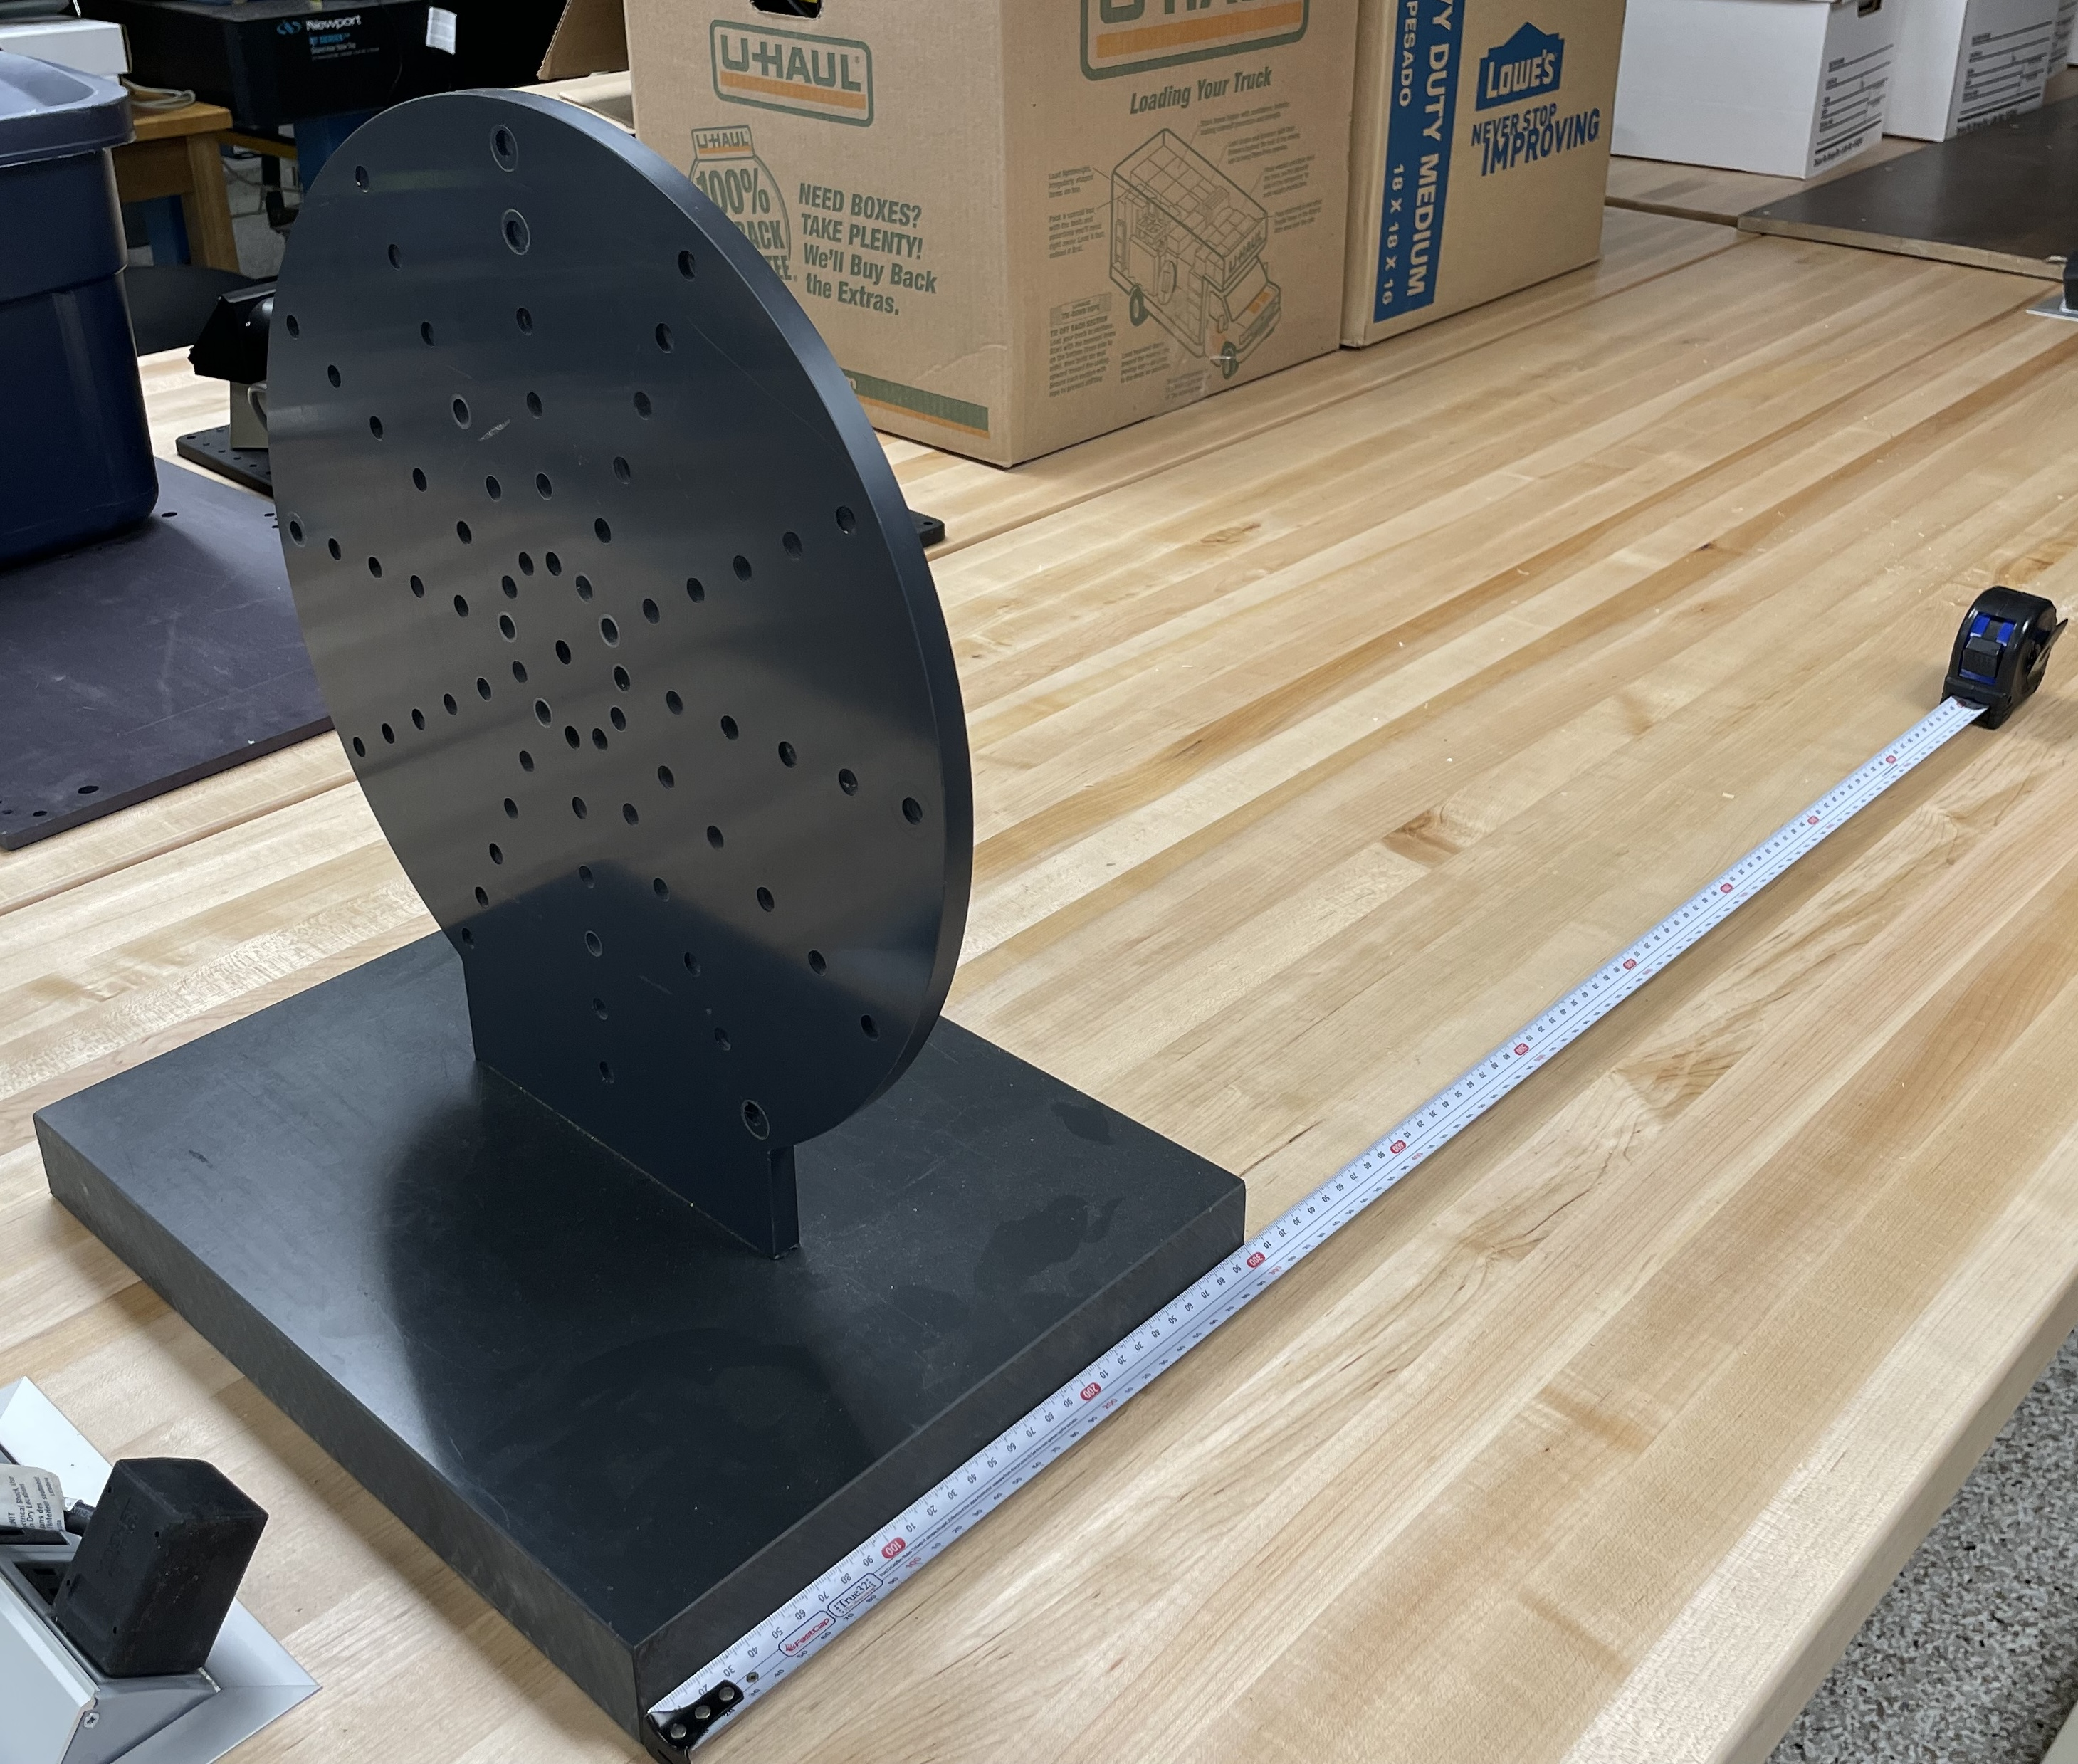
\includegraphics[width=\textwidth]{Assests/Picture3.jpg}
		\caption*{(a) PVC-based mapping platform.}
	\end{minipage}%
	\hfill
	\begin{minipage}[t]{0.48\textwidth}
		\centering
		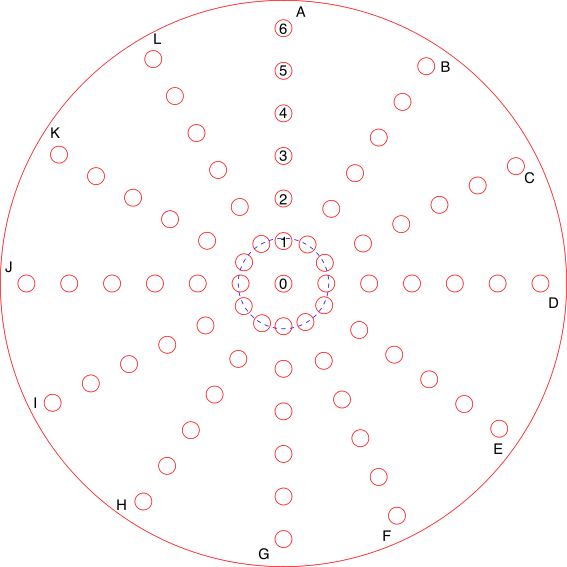
\includegraphics[width=0.85\textwidth]{Assests/MagFieldMap.png}
		\caption*{(b) Example field map output from MRI fringe region.}
	\end{minipage}
	\caption{PVC-based magnetic field mapping platform used for spatial $B_0$ and $\nabla B_0$ measurement. As shown in Ferreira 2017 \cite{haddixProposal,ferreira2017}.}
	\label{fig:fieldmapping}
\end{figure}


%LABVIEW program and Alpha Labs Protocols
Once the field‑mapping phantom and Gaussmeter probe are co‑aligned, data capture was streamlined to be sufficiently flexible and precise for our proximity measurements near an \gls{mri}. The manufacturer’s default software, AlphaApp, provides basic data‑logging, tethered or standalone recording, live screen streaming, and plotting of measurements from USB‑enabled AlphaLab meters\cite{AlphaApp}. However, AlphaApp **does not expose control over sampling frequency or allow real‑time adjustment of acquisition parameters**, limiting fine‑grained temporal resolution when the probe is moved into steep field gradients. In contrast, using \gls{lvi} interface allows for configurable sampling intervals, buffer control, and precise timing protocols, enabling us to push the device for much higher accuracy as the probe approaches and crosses isocontour regions within the \gls{mri} fringe. We developed that VI by leveraging the AlphaLab Data Acquisition Communication Protocol to command the device directly via USB, providing deterministic control over timing and sample rate \cite{AlphaAppProtocol}.

The data acquisition procedure for magnetic flux mapping is organized in this \gls{lvi}, whose basic logic is summarized in Figure~\ref{fig:gaussmeter-flowchart}. Upon startup, the \gls{lvi} initializes serial communication with the Gaussmeter, loads user-defined parameters (such as file name, mode of acquisition, delay time, and probe coordinates), and clears buffers in preparation for logging. The user may select either a continuous or an individual sampling mode. In continuous mode, the VI iterates through a defined number of data points with a fixed delay between samples; in individual mode, each data capture is triggered manually, allowing for precise positioning or timing. For both modes, each cycle involves reading the spatial coordinates, sending a measurement command, recording the returned magnetic flux value, and updating a graphical display as well as the output file.

While the flowchart reflects the core logic, it does not fully convey the customization added to the \gls{lvi} interface. For example, the front panel includes input fields for patient table (couch) parameters such as couch speed and displacement points. As mentioned above, our phantom is discretized with radial and angular indices: angular positions span 12 sectors clockwise from the 12 o’clock position (0 to 11 or A to L), and radial depths range from the center (0) to the outer edge (6). The probe’s spatial location is represented in polar coordinates, and the system plots magnetic flux as a function of position rather than time, allowing for intuitive visualization of the MRI fringe field across the phantom surface.

\begin{figure}[H]
	\centering
	\begin{tikzpicture}[node distance=1.5cm, every node/.style={transform shape}, scale=0.6]
	
	% Start
	\node (start) [startstop] {Start VI};
	
	% Initialization
	\node (initserial) [process, below of=start] {Initialize serial port (COM3, 115200 baud)};
	\node (readinput) [process, below of=initserial] {Read user inputs (file name, mode, delay, coords)};
	\node (clearbuf) [process, below of=readinput] {Clear buffers and arrays, create CSV};
	
	% Mode decision
	\node (mode) [decision, below of=clearbuf, yshift=-0.5cm] {Data collection mode?};
	
	% Individual branch: manual trigger wait before data steps
	\node (manualTrigger) [process, left=3.5cm of mode] {Wait for manual trigger};
	
	%Continuous loop
	\node (loopCount) [process, below =3cm of mode] {Loop: For i = 1 to N points};
	
	% Data acquisition steps (common)
	\node (readcoords) [process, below of=loopCount] {Read MRI coordinates (x,y,z)};
	\node (sendcmd) [process, below of=readcoords] {Send command to Gaussmeter};
	\node (readflux) [process, below of=sendcmd] {Read flux data (time, flux, error byte)};
	\node (store) [process, below of=readflux] {Append to arrays and CSV};
	\node (updateplots) [process, below of=store] {Update XY graph and polar plot};
	\node (checkerrors) [process, below of=updateplots] {Check for errors};
	
	% Continuous mode: wait delay after error check
	\node (delayWait) [process, below of=checkerrors, yshift=-1cm] {Wait preset delay};

	
	% Loop decision
	\node (moreRuns) [decision, below of=delayWait, yshift=-0.5cm] {More runs/points?};
	
	% End
	\node (end) [startstop, below of=moreRuns, yshift=-1cm] {End VI};
	
	% Arrows: initialization flow
	\draw [arrow] (start) -- (initserial);
	\draw [arrow] (initserial) -- (readinput);
	\draw [arrow] (readinput) -- (clearbuf);
	\draw [arrow] (clearbuf) -- (mode);
	
	% Mode branches
	\draw [arrow] (mode) -- node[above] {Individual} (manualTrigger);
	\draw [arrow] (mode) -- node[above] {Continuous} (loopCount);
	
	% Individual flow to data steps
	\draw [arrow] (manualTrigger) |- (readcoords.west);
	
	% Data acquisition common flow
	\draw [arrow] (loopCount) -- (readcoords);
	\draw [arrow] (readcoords) -- (sendcmd);
	\draw [arrow] (sendcmd) -- (readflux);
	\draw [arrow] (readflux) -- (store);
	\draw [arrow] (store) -- (updateplots);
	\draw [arrow] (updateplots) -- (checkerrors);
	
	% Continuous flow: after errors wait delay, then loop decision
	\draw [arrow] (checkerrors) -- (delayWait);
	\draw [arrow] (delayWait) -- (moreRuns);
	
	% Individual flow: after errors go directly to loop decision (skip delay)
	\draw [arrow] (checkerrors.east) -- ++(1,0) node[pos=0.3, right, xshift=20pt] {Individual only} |- (moreRuns.north);

	% Loop decision arrows:
	% If yes, loop back to the start of the mode branch
	% Intermediate branch point for Yes
	\node (yesBranch) [coordinate, left=2.5cm of moreRuns.west] {};
	
	% Arrow from moreRuns to yesBranch labeled "Yes"
	\draw [arrow] (moreRuns.west) -- node[midway, above] {Yes} (yesBranch);
	
	% Branch to Individual
	\draw [arrow] (yesBranch) -- node[pos=0.85,above] {Individual} ++(-7,0) |- (manualTrigger.west);
	
	% Branch to Continuous
	\draw [arrow] (yesBranch) -- node[pos=0.8,below] {Continuous} ++(-3,0) |- (loopCount.west);


	
	% If no, end program
	\draw [arrow] (moreRuns.east) -- node[midway, above] {No} ++(3,0) |- (end.east);
	
\end{tikzpicture}
	\caption{Flowchart of the Gaussmeter VI data acquisition algorithm.}
	\label{fig:gaussmeter-flowchart}
\end{figure}

In clinical use, the entire fixture is intended to be shifted axially along the Z-direction of a horizontal bore MRI scanner using controlled couch increments (e.g., 10 cm). This translation allows for volumetric sampling of $B_0$ over several planes. The spatial magnetic field gradient$\nabla B_0$ can then be estimated numerically using finite difference calculations between adjacent measurement points. This method has previously been applied to MRI mapping in the work by Ferreira \cite{ferreira2017}.





\subsection{Translational Force Measurement via Angular Deflection}

\subsubsection{Laboratory Simulation with Solenoid Coil}

To assess MRI-induced translational forces in a laboratory environment, Creighton University developed a pendulum-style apparatus following the geometry and physics outlined in ASTM F2052-15\cite{astmF2052}. The vertical post includes a screw clamp mechanism that enables height adjustment; however, a default suspension height of 1 meter was used for consistency across trials.

The experimental frame was constructed entirely from \gls{pvc} components (Figure \ref{fig:schematic}a), including a vertical post of 1.5 meters and a rigid base for stabilization. The sample—a \textbf{solid ferromagnetic cylinder} (length = 6 mm, diameter = 3 mm, mass = 0.3648 g, density = 8.6 g/cm$^3$)—was suspended by a \textbf{955 mm-long sewing thread}, tied via a simple knot at its center. For clinical applications, a \textbf{0.25 mm nylon monofilament} is recommended for improved reproducibility and safety. A Monofilament Nylon thread has low stretch,  complies with MR-safe properties (Non-metallic, Non-conductive, Non-magnetic), and reduces variability introduced by torsional drift or thread elasticity  \cite{stoianovici2024, astmF2052}. The bottom of the sample was free to swing, forming a pendulum under gravity. A horizontal ruler, fixed along the Z-axis, served as the visual reference to quantify lateral displacements as shown in Figure \ref{fig:schematic}b and detailed in Figure~\ref{fig:leadcloseup}. 


\begin{figure}[H]
	\centering
	\begin{minipage}[b]{0.48\textwidth}
		\centering
		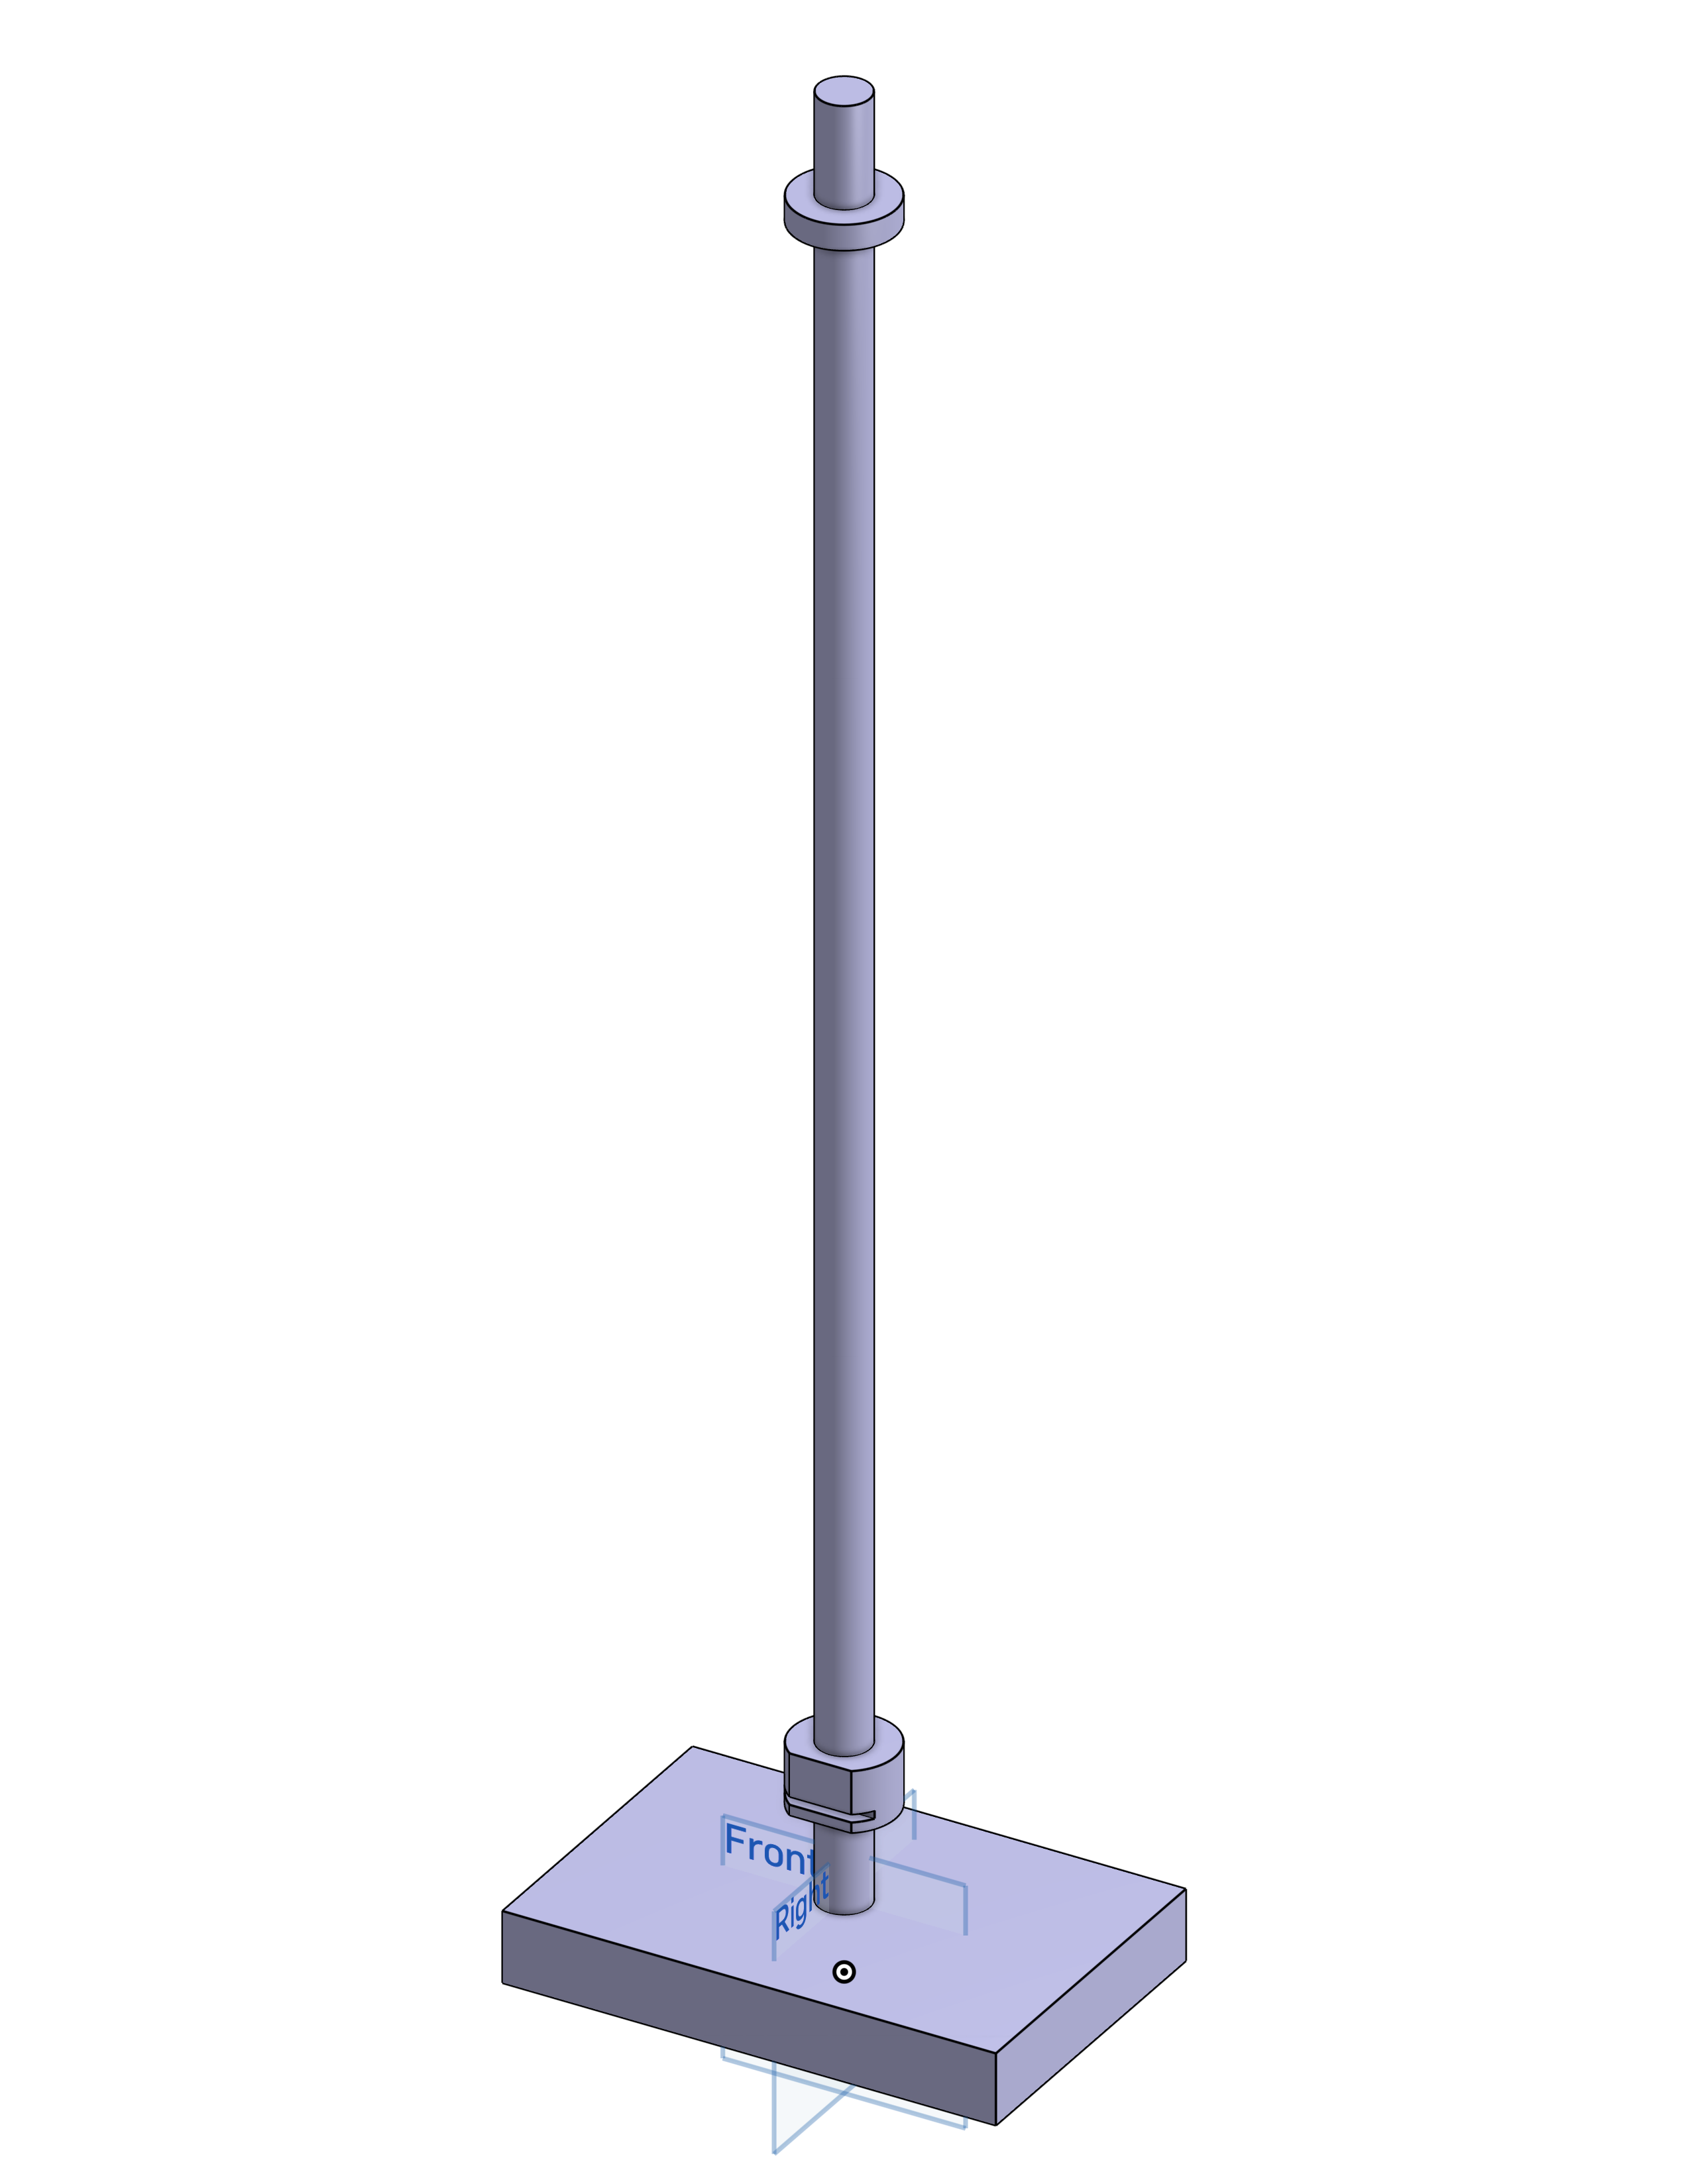
\includegraphics[width=\textwidth]{Assests/Part1.png}
		\subcaption{CAD render of the pendulum apparatus created using CATIA.}
	\end{minipage}
	\hfill
	\begin{minipage}[b]{0.48\textwidth}
		\centering
		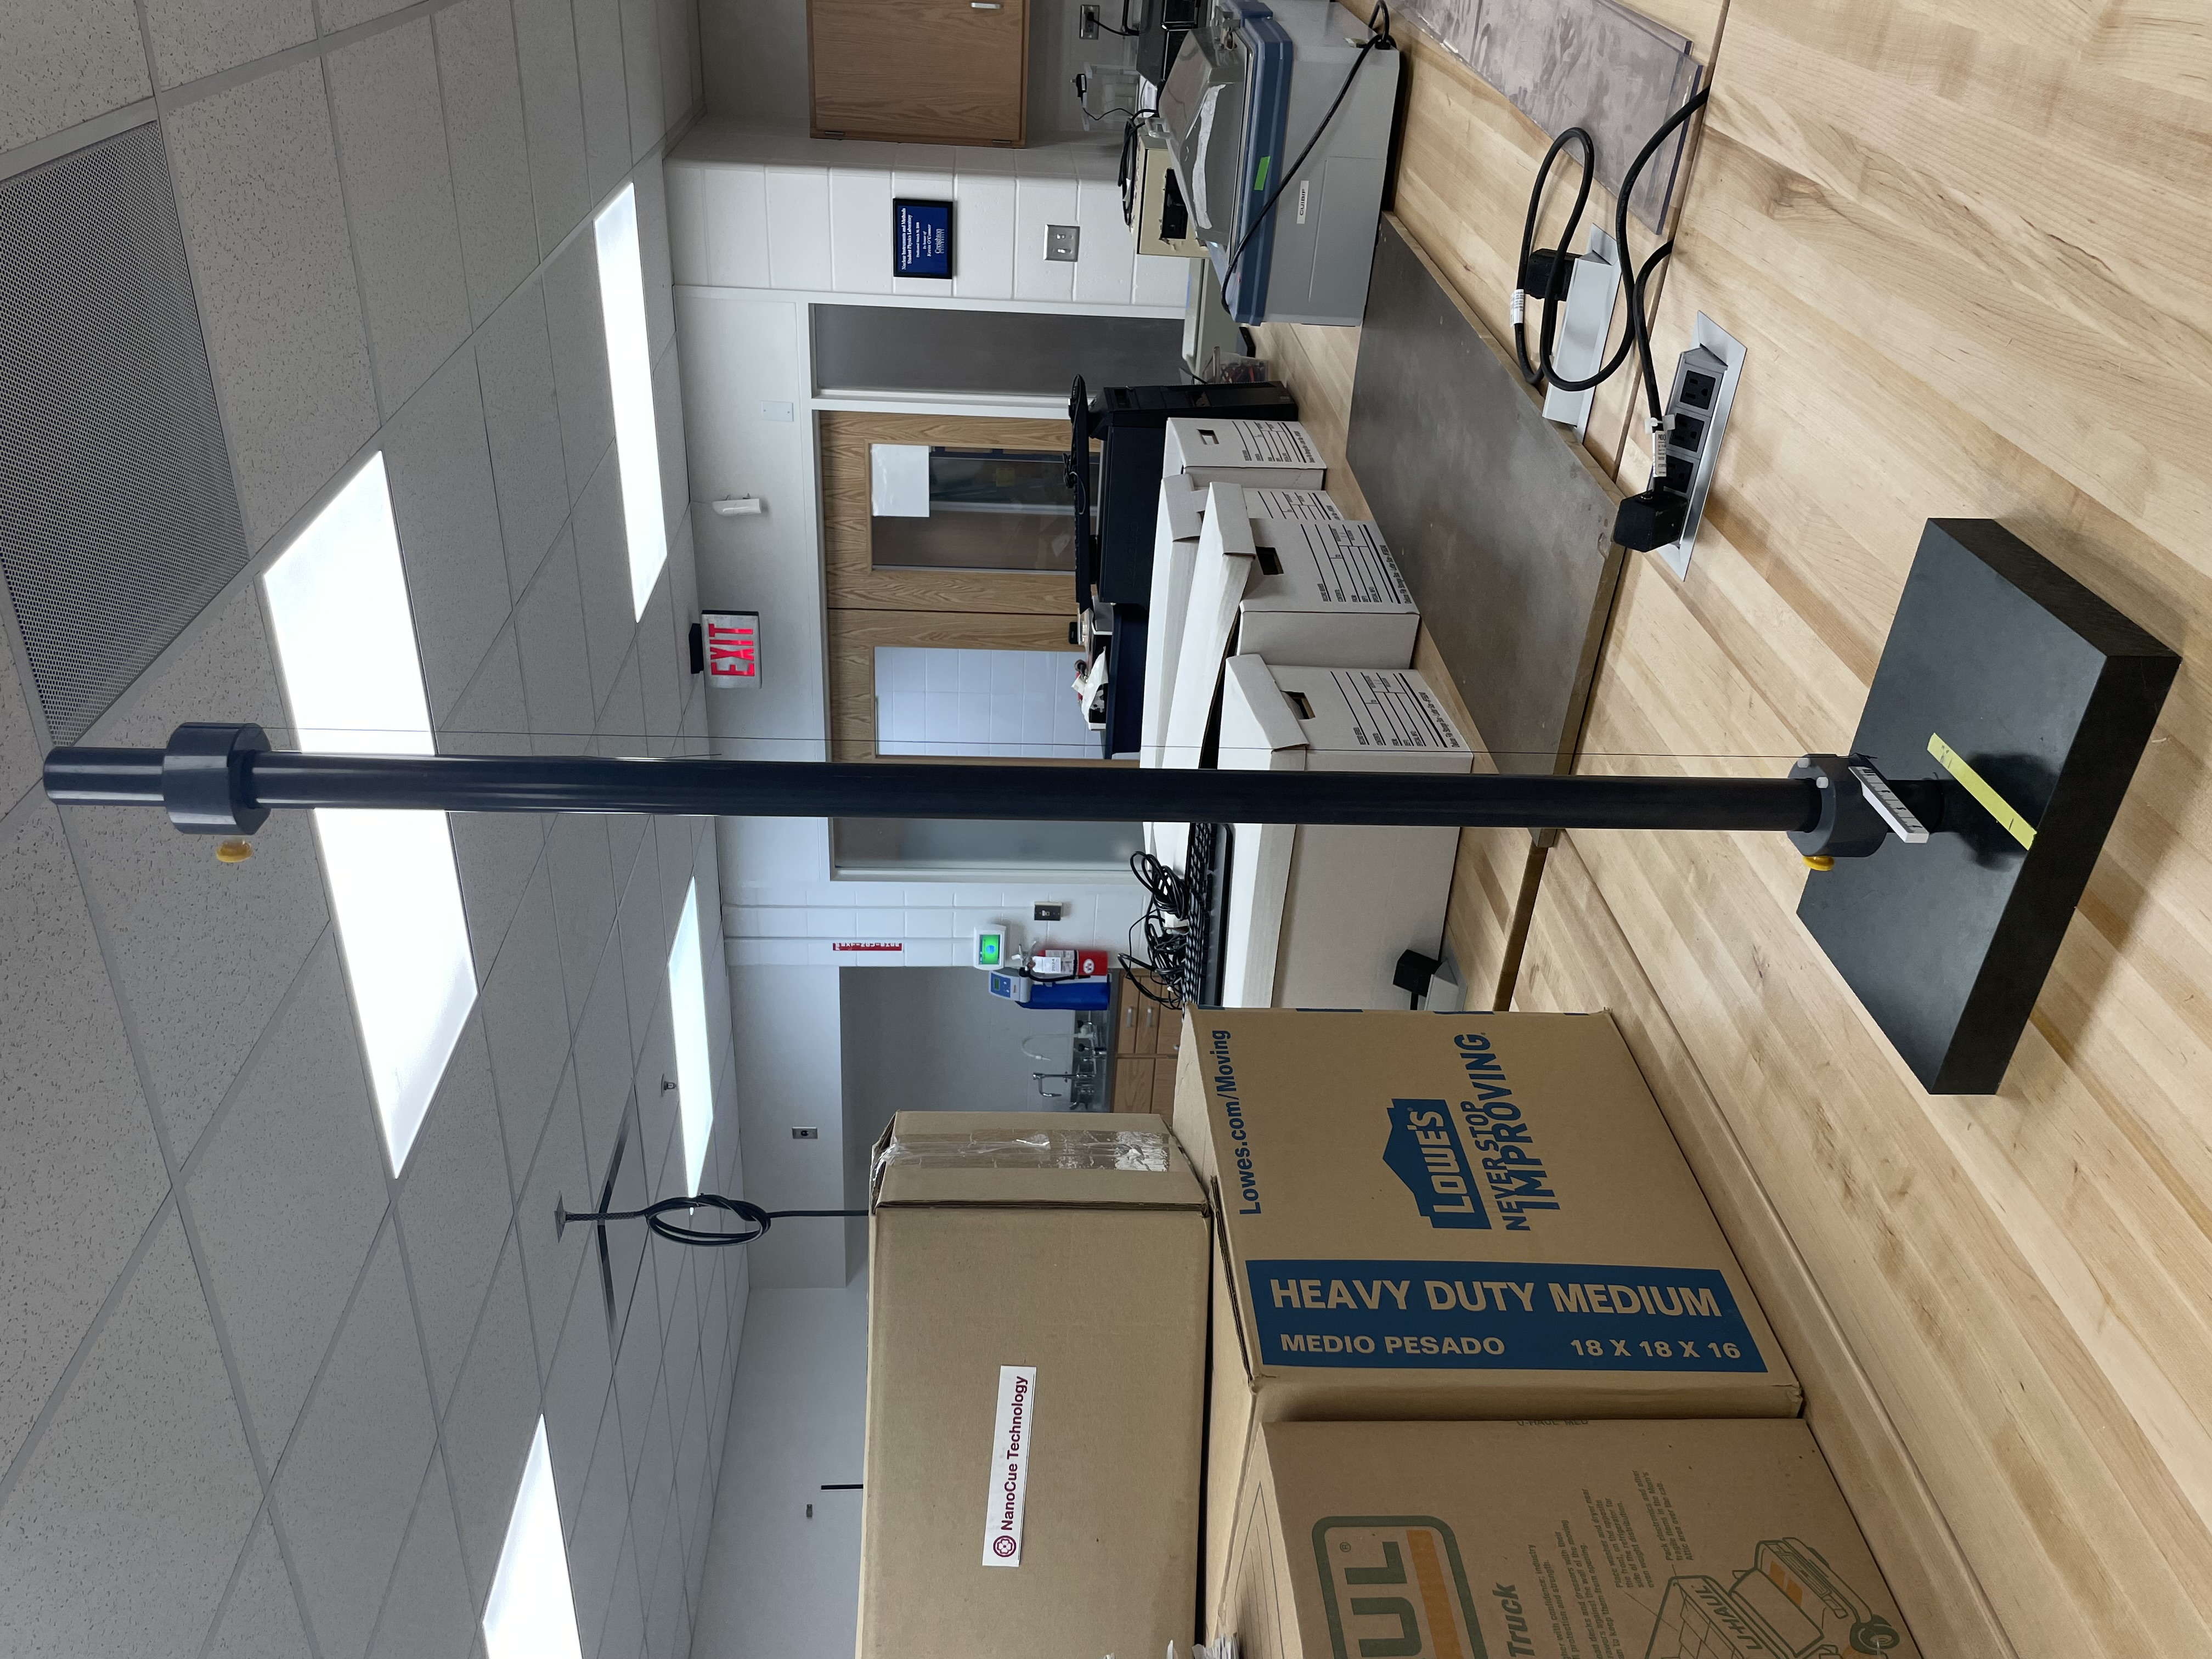
\includegraphics[width=1.3\textwidth, angle=-90]{Assests/Picture1.jpg}
		\subcaption{Real-life implementation of the apparatus in the laboratory setting.}
	\end{minipage}
	\caption{Experimental pendulum-based apparatus constructed from PVC for MRI translational force measurements.}
	\label{fig:schematic}
\end{figure}

\subsubsection*{Lead Holder Frame Design}

To accommodate epicardial lead positioning while maintaining MRI compatibility, we propose the use of a lightweight, non-magnetic bee comb mesh also fabricated from \gls{pla}. The suggested mesh dimensions are 16 mm length by 14 mm wide, with a thickness of 1 mm, for a total volume of less than $100 mm^3$ equivalent to around a tenth of 1 gram given the 1.24 grams per cubic centimeter ($g/cm^3$) \gls{pla} density. 

As shown in figure \ref{fig:leadHolder} and \ref{fig:leadcloseup}.

The mesh needs to be suspended such that the lead axis was aligned approximately parallel to the magnetic field gradient (Z-axis). The mesh's lightweight design aimed to minimize its contribution to the total magnetic force, however its mass was not explicitly subtracted from the translational force calculations.

\begin{figure}[H]
	\centering
	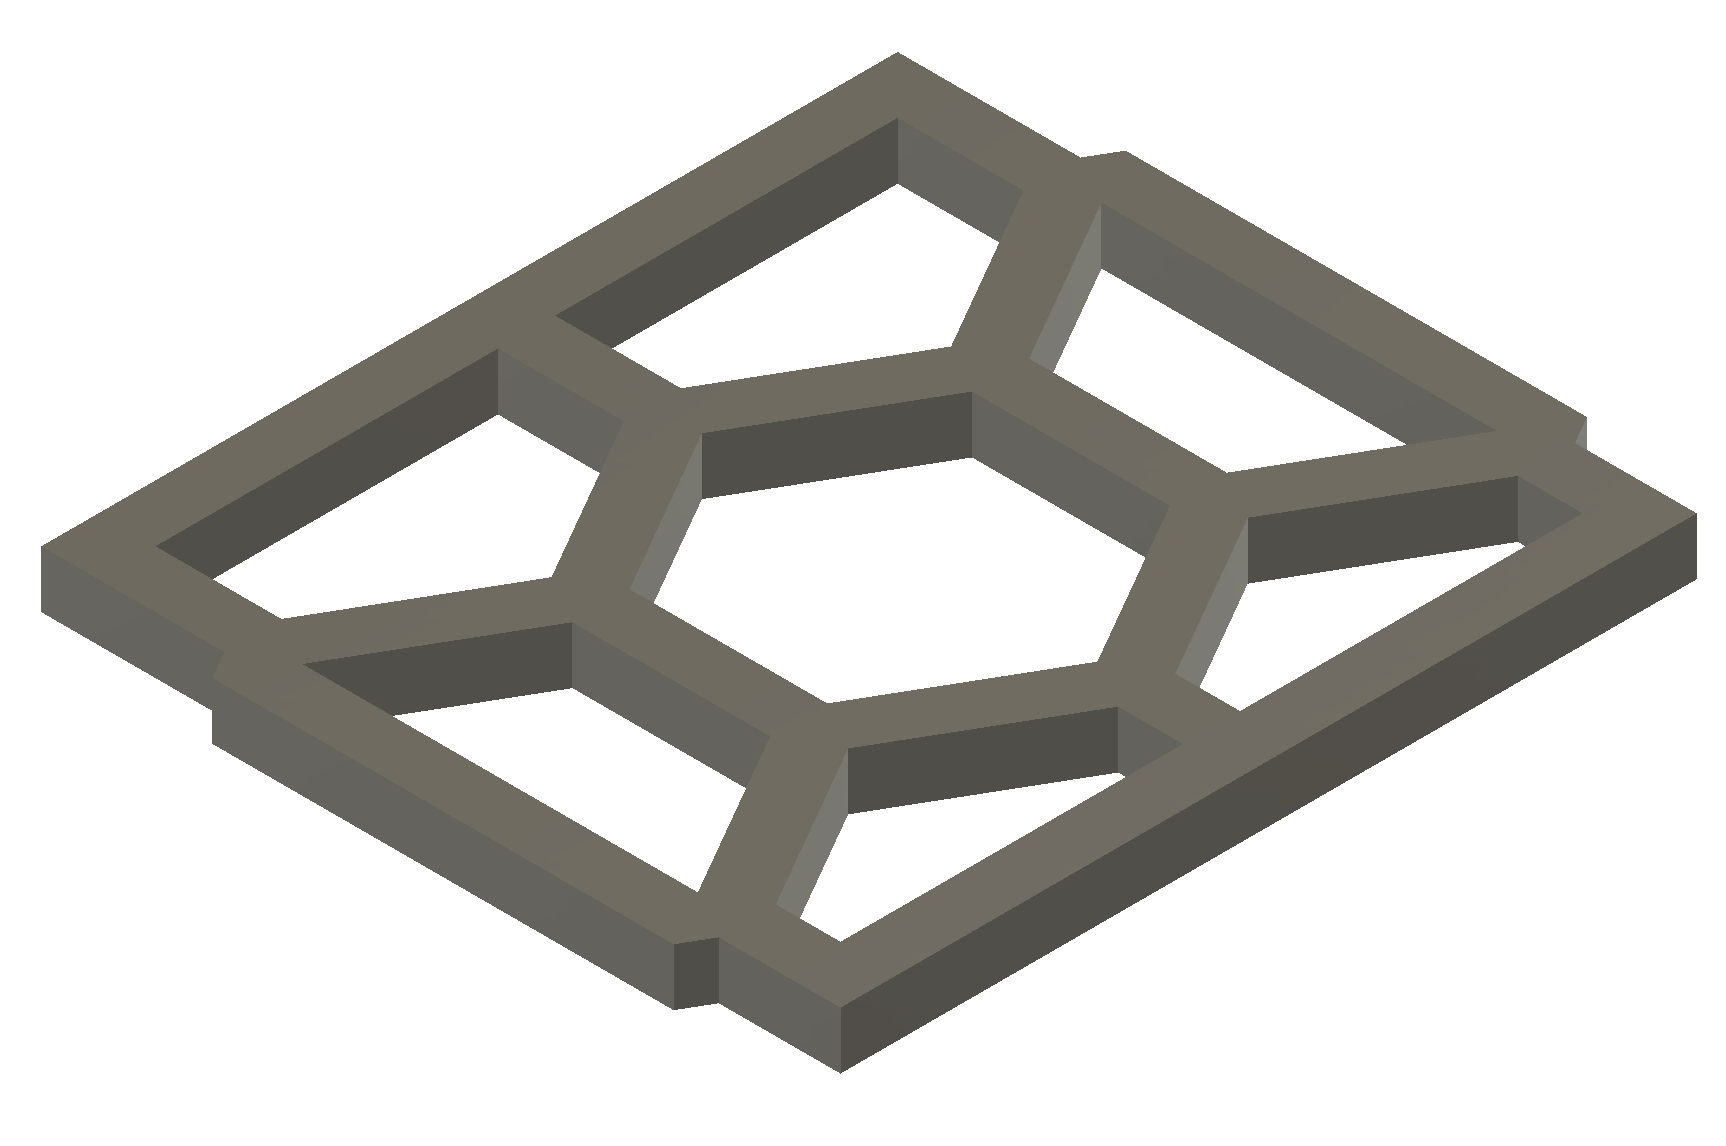
\includegraphics[width=0.5\textwidth]{Assests/frameHolder.png}
	\caption[3D render of the design on lead holder]{The design on lead holder comprises a rectangular lightweight bee comb mesh to wrap the epicardial lead around and hold it in a pendulum with a nylon string}	
	\label{fig:leadHolder}
\end{figure}

A summary schematic of the apparatus and frame are included in Figures \ref{fig:schematic} and \ref{fig:leadHolder}, with additional engineering drawings available in %\textbf{\AppendixAone} and \textbf{\AppendixAtwo}.



\begin{figure}[H]
	\centering
	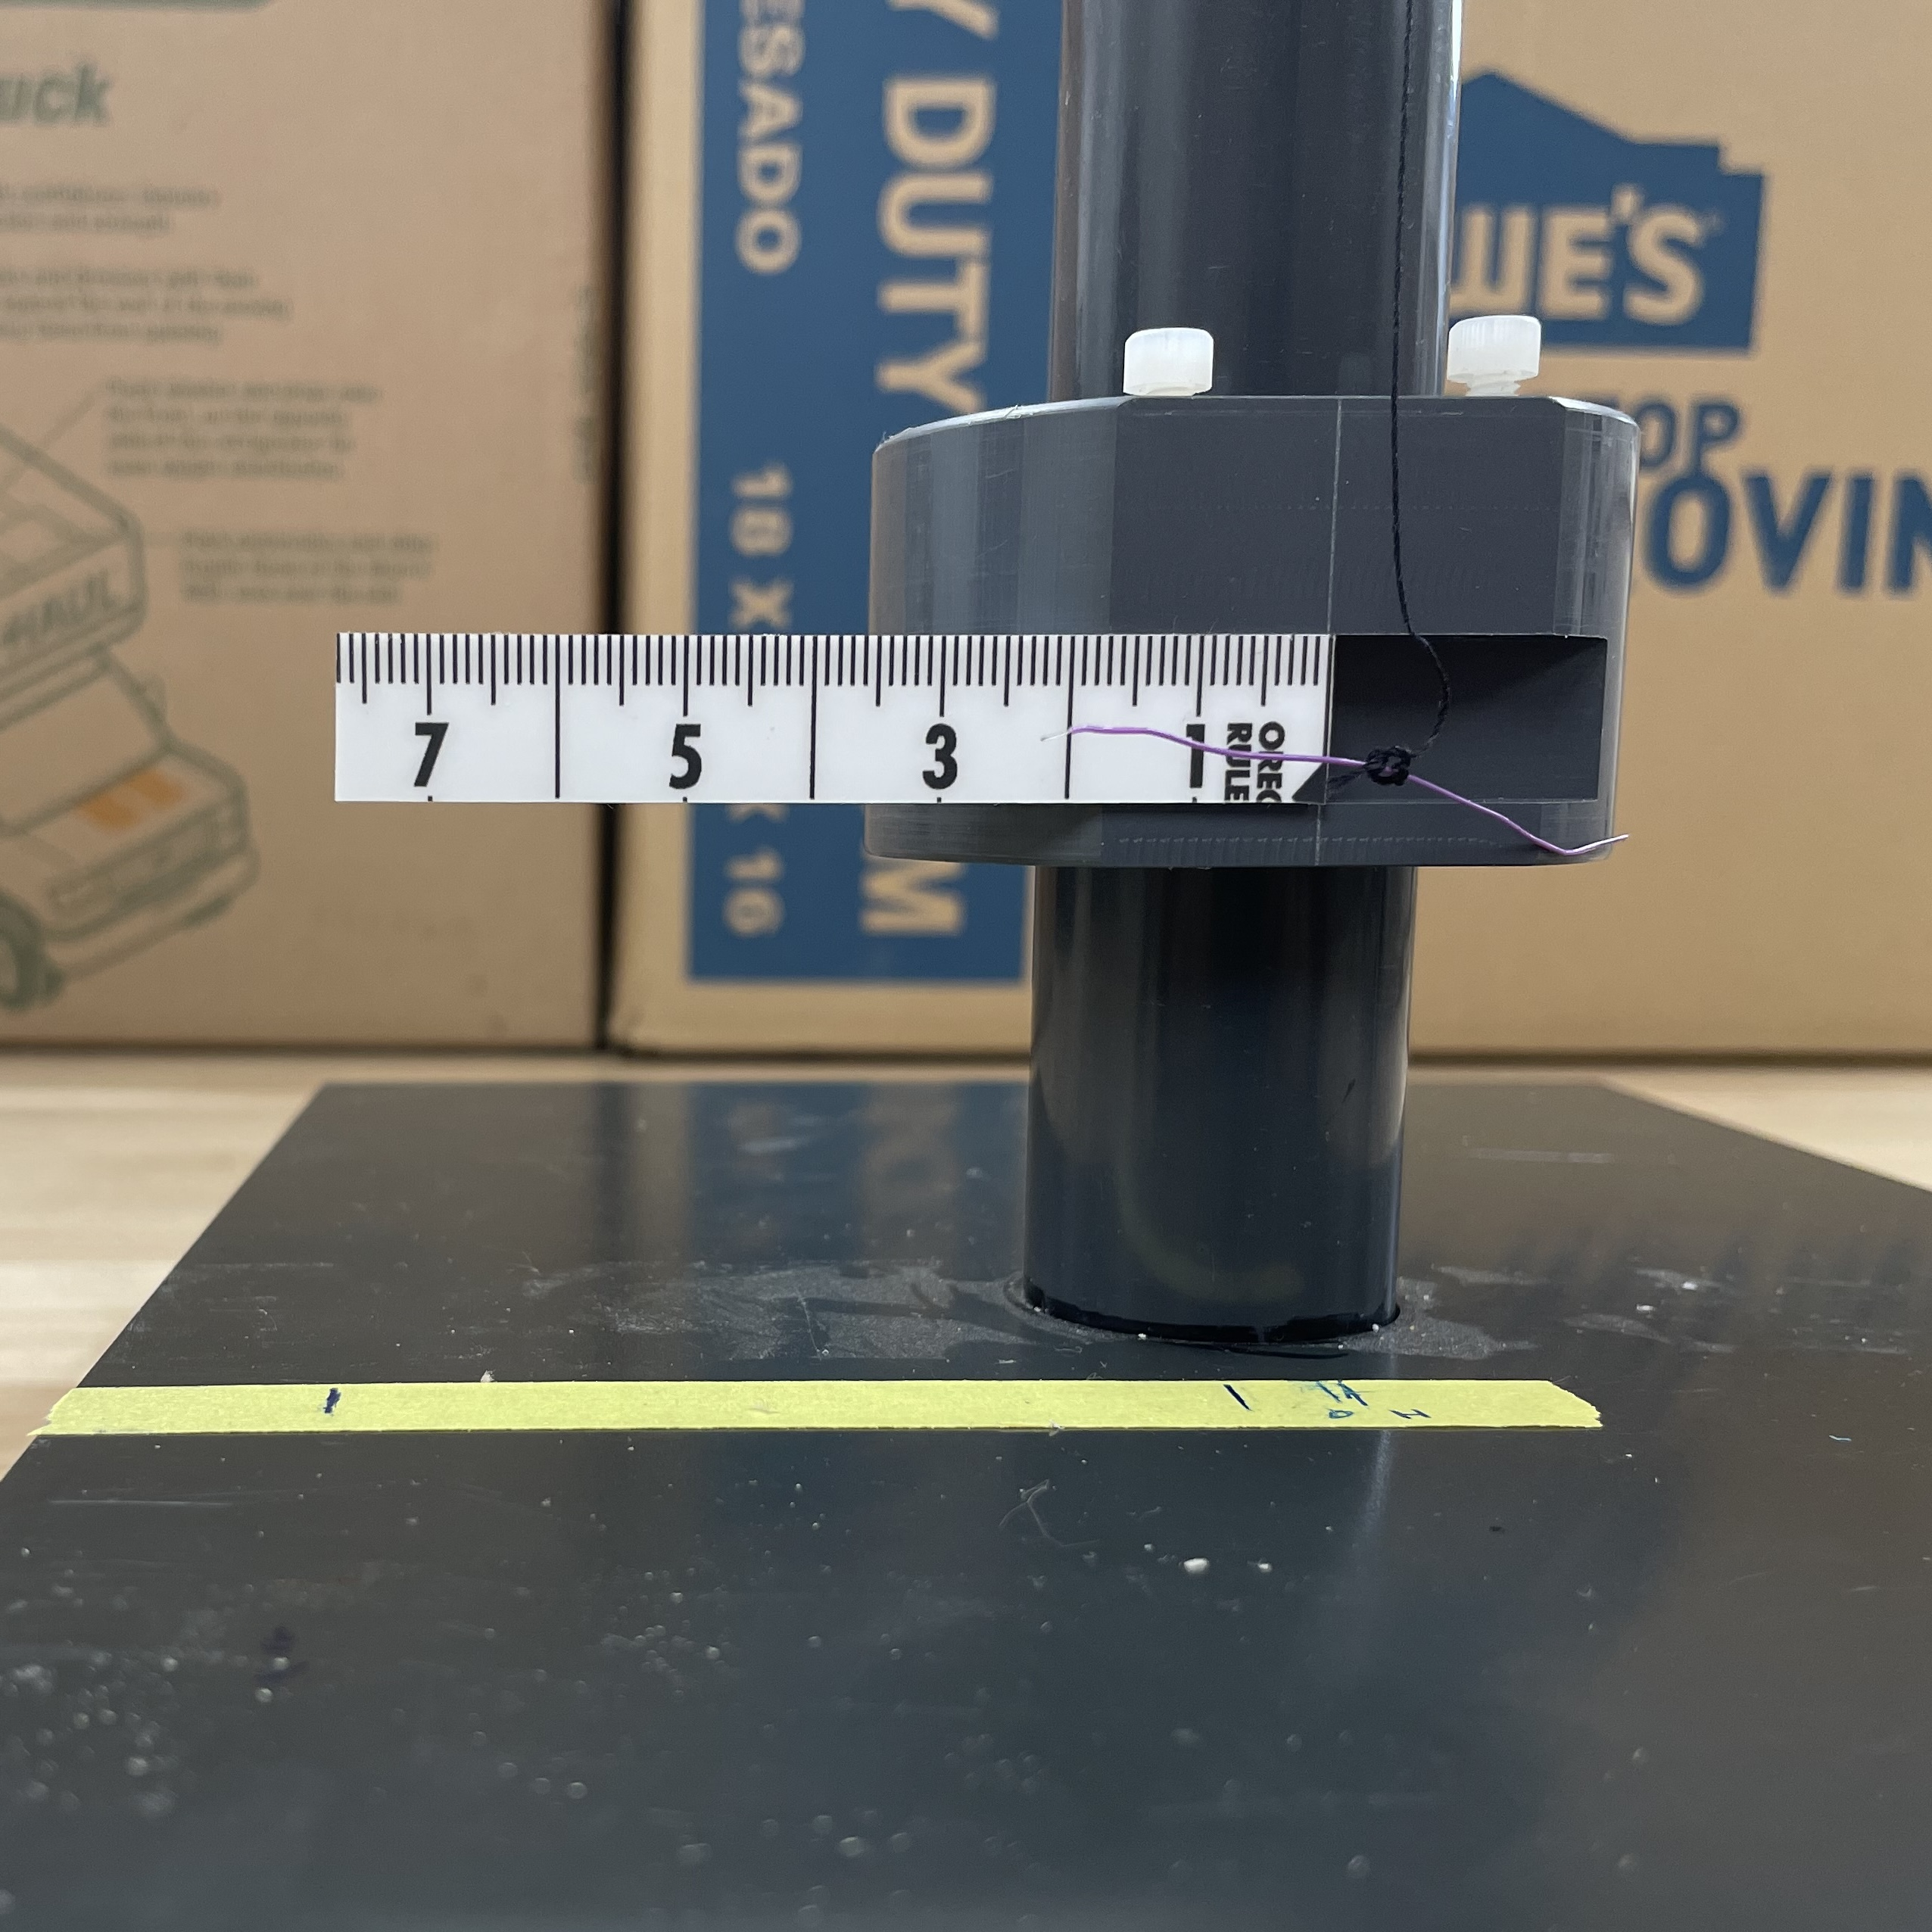
\includegraphics[width=0.6\textwidth]{Assests/Picture2.jpg}
	\caption{Close-up of the epicardial lead fragment suspended by monofilament thread over the ruler. Image illustrates the displacement measurement system and the sample scale.}
	\label{fig:leadcloseup}
\end{figure}

\subsubsection*{In Lab Measurement Protocol}

Magnetic field measurements were performed using the \textbf{AlphaLab Inc. Gaussmeter} described before. To characterize local field gradients, measurements were taken at three positions: at the pendulum's equilibrium position, 0.5 mm below, and 0.5 mm above, yielding values of $B_{-0.5}$, $B_0$, and $B_{+0.5}$, respectively. Each position was sampled \textbf{nine times per current level}, and gradients were computed using python pandas library and the central finite difference method:

\begin{equation}
	\frac{dB}{dz} \approx \frac{B_{+0.5} - B_{-0.5}}{1\ \text{mm}}
\end{equation}

Once the pendulum reached equilibrium under each magnetic condition, the horizontal displacement on $z$ was recorded visually using the ruler as a reference. With known suspension length $L$, the \textbf{deflection angle $\alpha$} was calculated as:

\begin{equation}
	\alpha = \tan^{-1}\left(\frac{x}{L}\right)
\end{equation}

Following ASTM F2052-15, the translational force exerted on a device due to a static magnetic field spatial gradient can be evaluated through angular deflection. In this setup, the test object is suspended in equilibrium, and the balance of forces leads to:

\begin{equation}
	\tan \alpha = \frac{F_m}{mg}
\end{equation}

where $\alpha$ is the deflection angle from vertical, $F_m$ is the magnetically induced translational force, $m$ is the mass of the object, and $g$ is the gravitational acceleration. Rearranging gives:

\begin{equation}
	F_m = mg \tan \alpha
\end{equation}

This is also derived from Newtonian force balancing as in Appendix X2 of ASTM F2052-15 (Fig \ref{fig:astm_diagram}), and is valid even in cases when the magnetic force does not operate exactly at the center of mass. As a result, the approach is reliable for evaluating a variety of devices.

\begin{figure}[htbp]
	\centering
	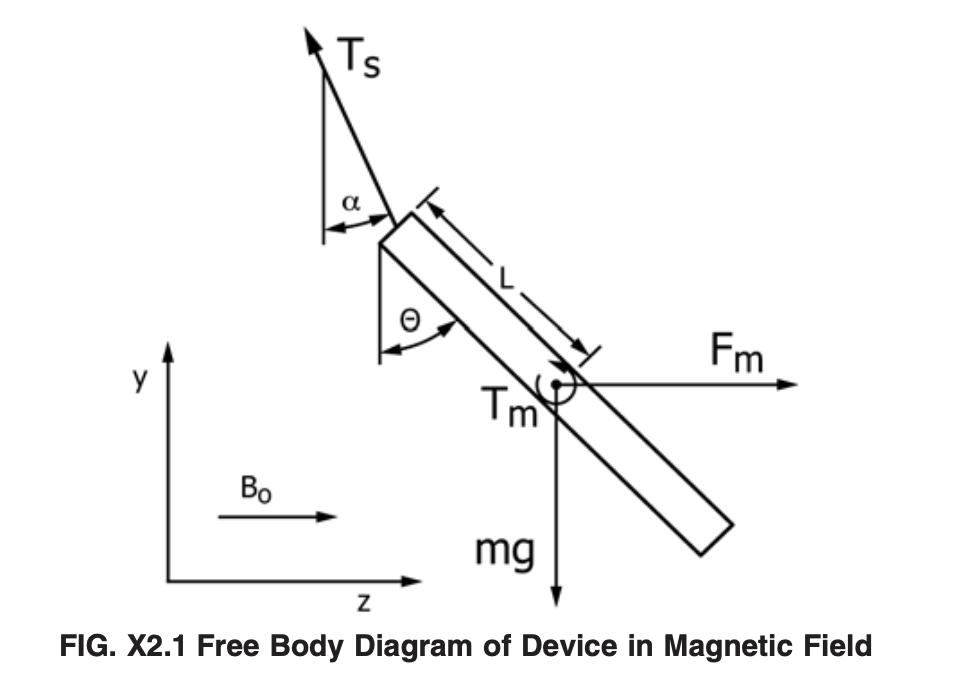
\includegraphics[width=0.6\textwidth]{Assests/astm_diagram.png}
	\caption{Free-body diagram of device in magnetic field (adapted from ASTM F2052-15, Appendix X2).}
	\label{fig:astm_diagram}
\end{figure}

For materials where magnetization is induced by a static field (e.g., paramagnetic or unsaturated ferromagnetic materials), the translational force can also be expressed in terms of volumetric magnetic susceptibility $\chi$, assuming linear response:

\begin{equation}
	F_m = \frac{\chi V}{\mu_0} B_0 \frac{dB_0}{dz}
	\quad \Rightarrow \quad
	\chi = \frac{\mu_0 F_m}{V B_0 \frac{dB_0}{dz}}
\end{equation}

Combining this with the earlier result:

\begin{equation}
	\chi = \frac{\mu_0 m g \tan \alpha}{V B_0 \frac{dB_0}{dz}}
\end{equation}

This provides a direct estimation of magnetic susceptibility from angular deflection measurements, provided the field and its gradient are known. 

The ratio is expressed as follows using a different, dimensionally reduced form from ASTM F2052-15's Appendix X3:

\begin{equation}
	\frac{\chi}{\rho \mu_0 g} = \frac{\tan \alpha}{B_0 \frac{dB_0}{dz}}
\end{equation}

This formulation explains why the measured deflection angle $\alpha$ (and thus $F_m$) depends not on $\chi$ or $B_0$ independently, but on their product. Practically, this insight justifies our lab methodology: although our solenoid generates only ~20 Gauss, we used a highly ferromagnetic sample (large $\chi$), allowing us to replicate clinically relevant force-to-weight ratios ($F_m / mg$).

In the clinical MRI environment, $B_0$ may reach 3 T, but the $\chi$ of implanted materials is often orders of magnitude smaller. This inverse balance preserves the translational force regime, and supports translating results from lab simulations to clinical conditions.

%\subsection*{Data Collection and Analysis}

All measurements were logged in \textbf{Microsoft Excel}, and photos/videos were captured via smartphone to document behavior. A minimum of \textbf{three trials} were performed for each current level; however, only the final (most consistent) dataset was retained for analysis. Data were exported to a Jupyter Notebook for clean up and processing with pandas. Then plotted to evaluate $\tan \alpha$ vs. field gradient force. Propagated uncertainties in $\alpha$ and $dB_0/dz$ were computed using standard error propagation formulas.

\subsubsection{In Clinic Measurement Protocol}




\subsection{Torque Measurement Apparatus (In Progress)}

A torque measurement system based on ASTM F2213 is under development. While a prototype was fabricated under the supervision of Dr. Nichols and prior students, detailed calibration, operational workflow, and data acquisition methods are still being finalized. The system is expected to allow both qualitative torque threshold assessments and quantitative torque calculation by assessing rotational displacement under a known static field. This device is shown in figure \ref{fig:torqueDevice}.


\begin{figure}[H]
	\centering
	\begin{minipage}[b]{0.48\textwidth}
		\centering
		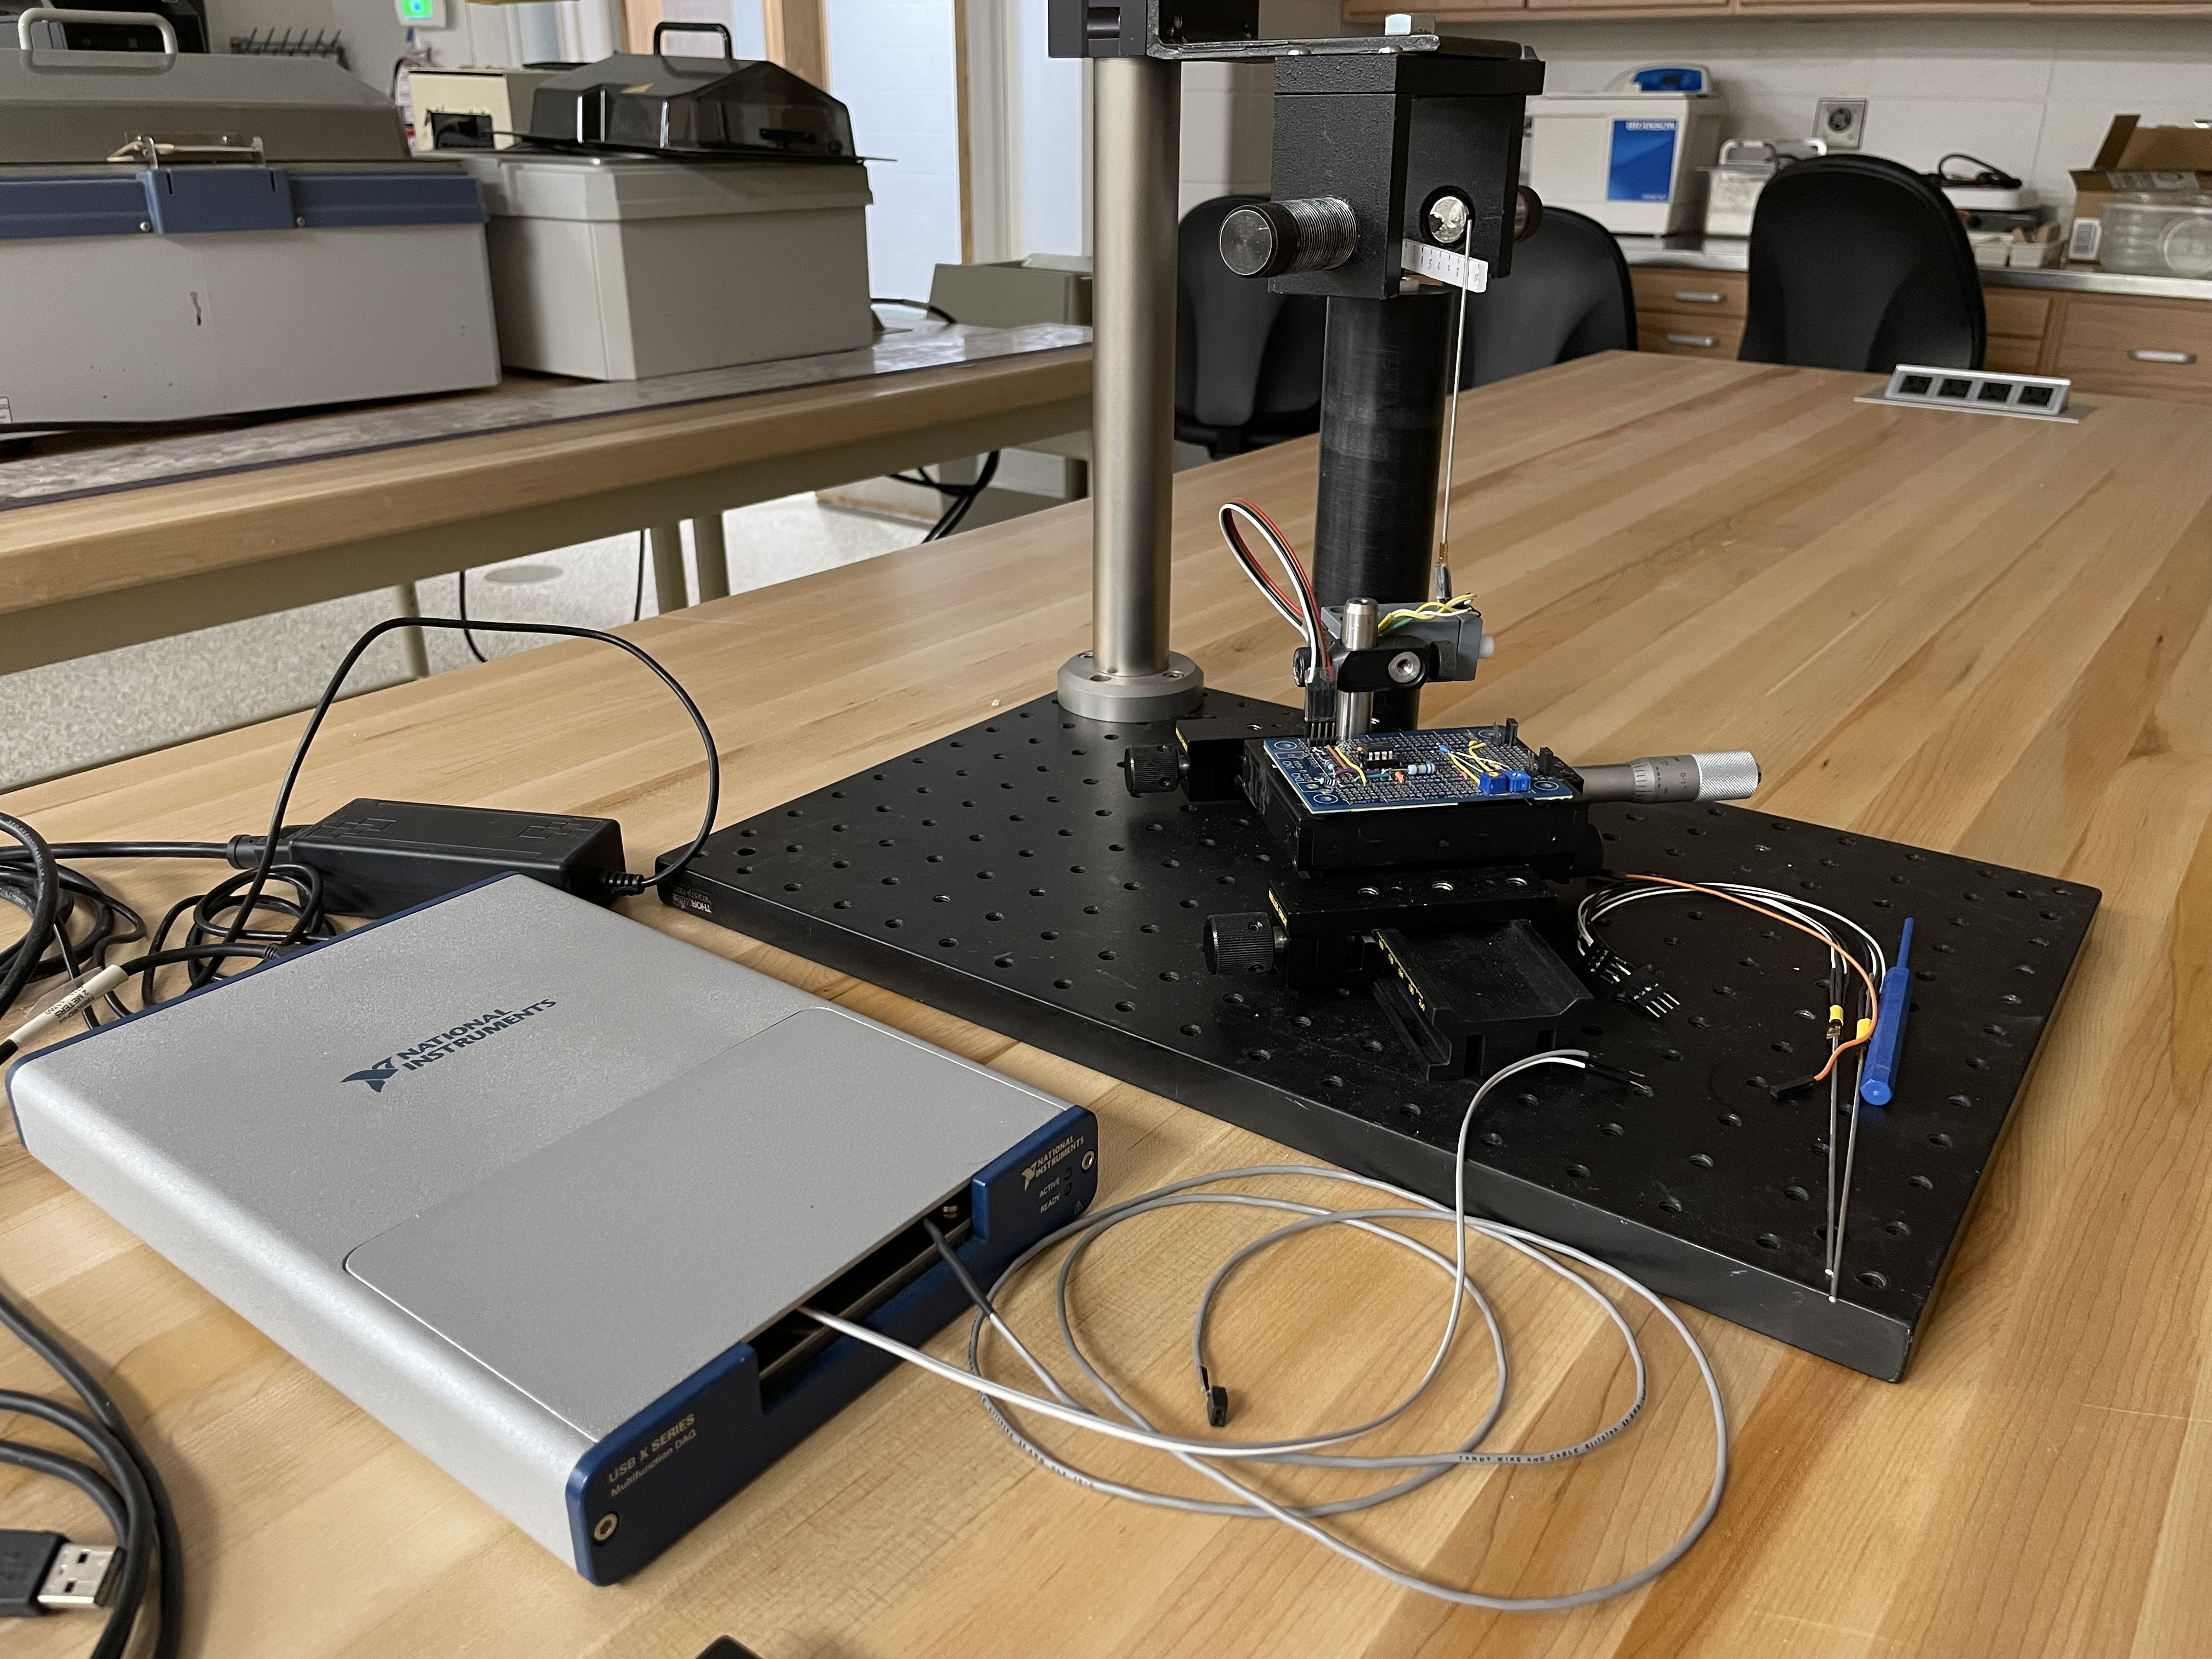
\includegraphics[width=\textwidth]{Assests/torquesDev.jpg}
		\subcaption{Current torque measurement device}
		\vspace{0.95cm}
	\end{minipage}
	\hfill
	\begin{minipage}[b]{0.48\textwidth}
		\centering
		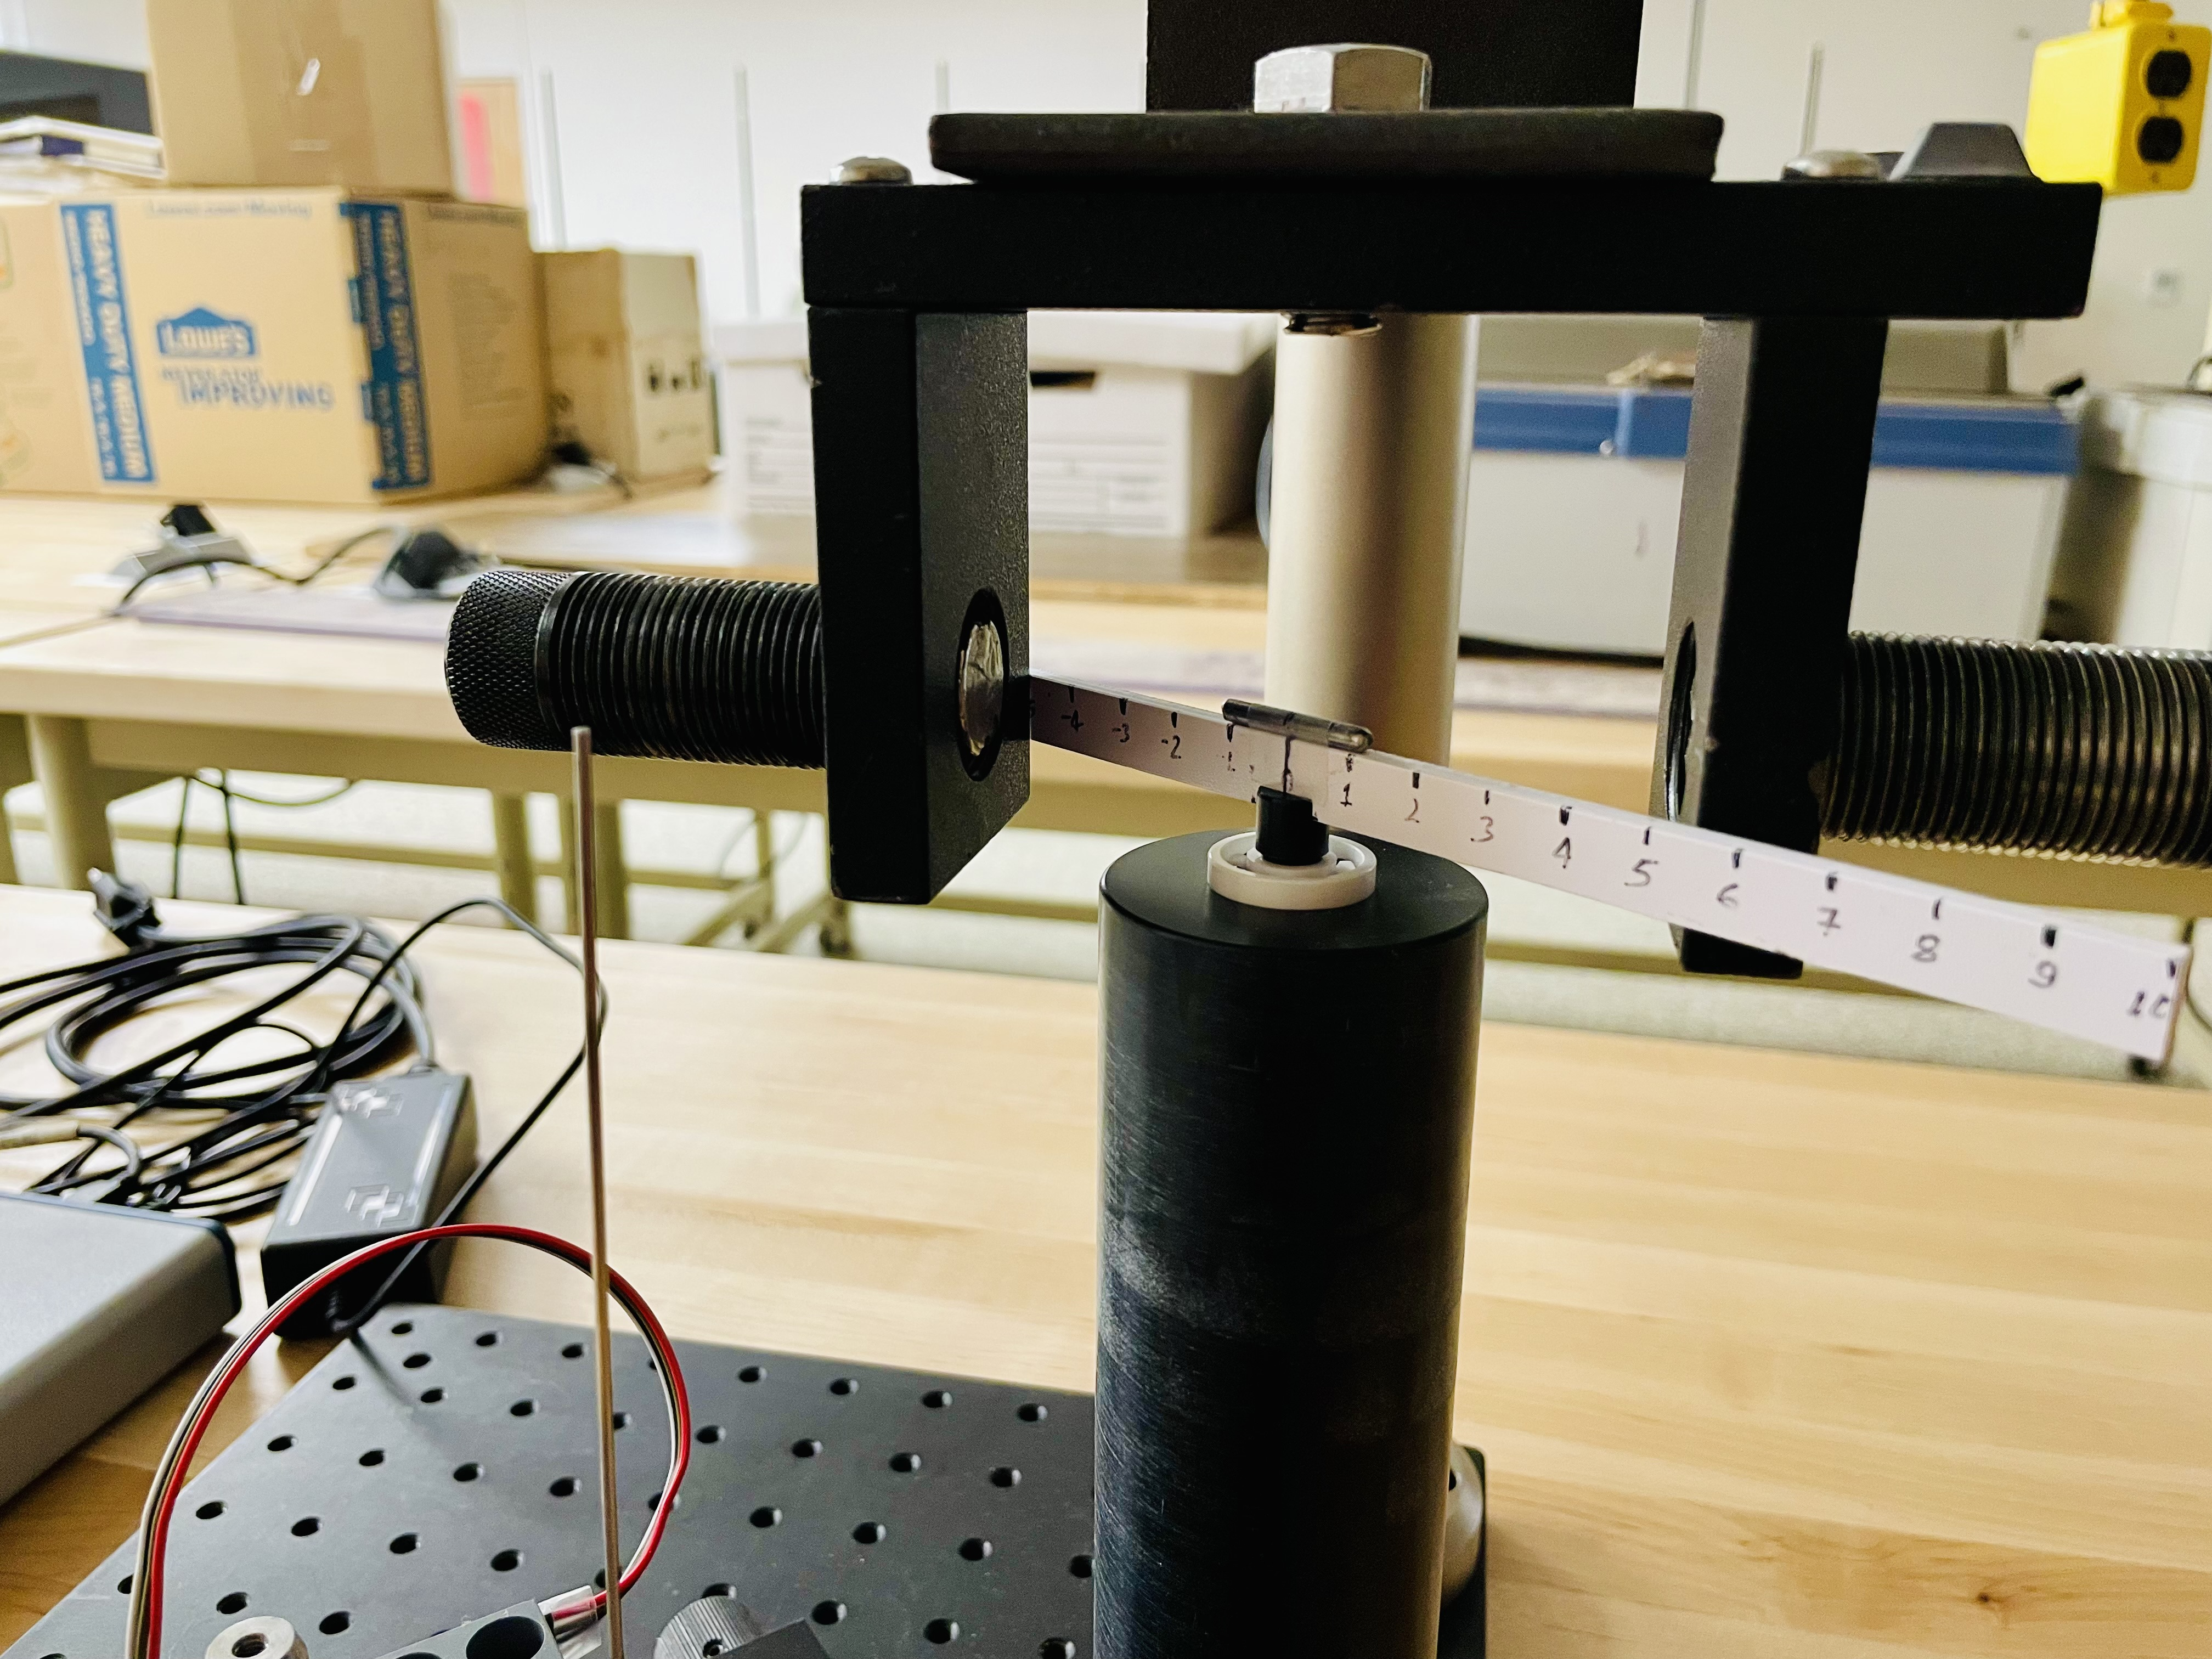
\includegraphics[width=\textwidth]{Assests/torquesCloseup.jpg}
		\subcaption{Close up to the neodymium magnets and test sample (cylindrical metallic piece) were torques are applied.}
	\end{minipage}
	\caption{Implementation of the apparatus in the laboratory setting.}
	\label{fig:torqueDevice}
\end{figure}

